%\todo{We have to improve this section- add a picture for workflow}
%\todo{Boris will do it}

In this section, we describe the workflow for reusing available vocabulary terms when building ontologies based on an existing catalogue of vocabularies. Recall that we do not specify which will be the expressivity of the resulting ontology. We foresee that the resulting ontology is likely to be a lightweight ontology. However the data publisher is responsible for adding more semantics when reusing existing vocabulary terms. Figure \ref{fig:workflow} depicts the proposed workflow. 

\begin{figure}
\centering
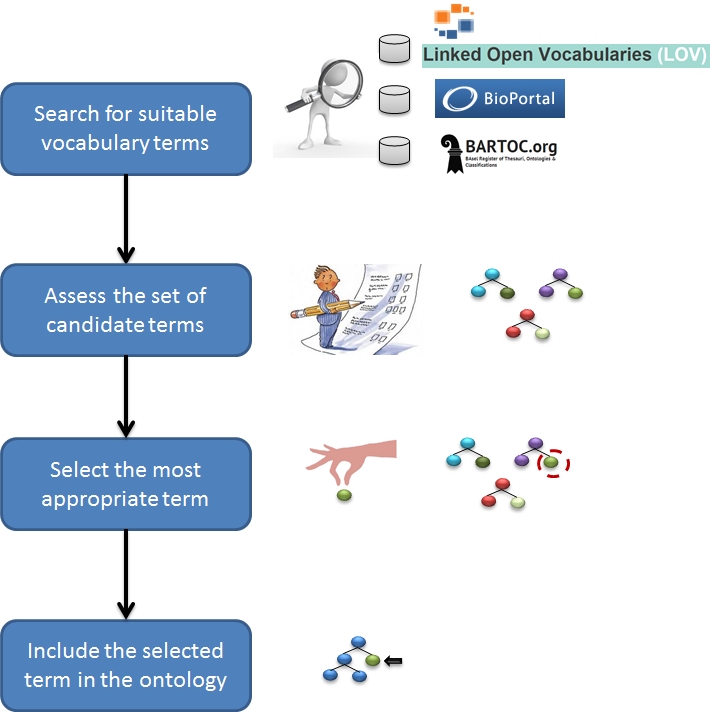
\includegraphics[scale=0.5]{./img/process}
\caption{Workflow for reusing available terms when building ontologies}
\label{fig:workflow}
\end{figure}


\begin{comment}
\subsection{Use case scenario: lobid vocabulary}
\label{lobid vocabulary}
Looking at the evolution of some vocabularies with highest changes since their release in LOV,\texttt{lobid} vocabulary is the winner with 16 modifications. The \texttt{lobid} vocabulary\footnote{\url{http://purl.org/lobid/lv}} is a vocabulary designed for the  linking open bibliographic data services. The ontology was first published on 2012-03-02 with only two properties, a minimal metadata information and labels in English. Since then, there have been 15 different versions and the current version (version of 2015-02-09) of the ontology contains 8 classes and 16 properties. Based on the different changes occurred during the on-going development of the lobid vocabulary, vocabulary changes can be grouped in two categories:
\begin{itemize}
\item Editorial changes (EDc) are the ones related with labels and comments translations, typos fixed. Those changes don't affect the structure of the vocabulary.
\item Semantic changes (SMc) are related with modifying the structure of the vocabulary, by either adding new axioms, new classes and properties.
\end{itemize}

Furthermore, the semantic changes can be broken down in four categories related to the main parts of a vocabulary, that are metadata, classes, properties and axioms. Thus we can group them as follows:

\begin{itemize}
\item Metadata changes (MTc), when the changes are related with the metadata section of the vocabulary. E.g., adding provenance information, license, publishers and creators data.
\item Property changes (PPc), when updating the vocabulary 
\item Classes changes (CLc), such as the creation of named classes.
\item Axioms changes (AXc) for updates using some axioms for restrictions in or the creation of anonymous classes. 

\end{itemize}

Table \ref{tab:lobid} summarizes the number of changes for the lobid vocabulary. In  a total of 20 changes, only 2 are editorial changes and each time accompanied with a semantic change in the corresponding version.
\texttt{lobid} vocabulary is a good example of reusing existing terms where the definition of all the classes are ``subclassing'' of three existing vocabularies: \texttt{dct}, \texttt{bibo} and \texttt{archives}\footnote{\url{http://data.archiveshub.ac.uk/def/}}.  

\begin{table}[!htb]
\centering{

\begin{tabular}{lccccc}
\hline
 \textbf{Changes} & EDc & MTc & PPc & CLc & AXc \\ \hline
  Numbers & 2 & 4 & 8 & 3 & 3 \\
 
 \hline
\end{tabular}
\caption{Changes observed in the lobid vocabulary since its release in 2012. }
\label{tab:lobid}
}
\end{table}

\end{comment}


%\subsection{Workflow on Reusing Terms}
In a nutshell, the activity of building vocabularies by reusing available vocabulary terms consists of the following tasks:

\begin{itemize}
	\item Search for suitable vocabulary terms to reuse from any vocabulary repository, such as BioPortal\footnote{\url{http://bioportal.bioontology.org/}}, LOV\footnote{\url{http://lov.okfn.org/}}, Bartoc.org\footnote{\url{http://bartoc.org}}, etc. The search should be conducted by using the terms of the application domain.
	\item Assess the set of candidate terms from the vocabulary repository. The goal of this task is to find out if the candidate terms are useful and relevant for the ontology being built. For this purpose we can rely on metrics provided by the vocabulary repository. In the particular case of LOV, the results include a score related to their ``importance'' in the corpus for each term retrieved. For every vocabulary in the LOV, terms (classes, properties, datatypes, instances) are indexed and a full text search feature is offered\footnote{\url{http://lov.okfn.org/dataset/lov/terms}}. The Linked Open Vocabularies search engine ranking algorithm takes  into account the popularity of the term within the LOV ecosystem and most importantly assigned a different score depending on which label property a searched term matched~\cite{vandenbusschelov}.		
	\item Select the most appropriate term taking into account the assessment task. To distinguish between those candidate terms which are the most suitable, we propose to use the following criteria (i) the stability of the URI namespace, (ii) the trustworthiness of the publisher of the vocabulary and (iii) the presence or absence of a community using the vocabulary. With respect to LOV repository we can also rely on the score of terms.
	\item Include the selected term in the ontology that has being developed. There are at least three alternatives in this case 
	\begin{itemize}
		\item Include the selected term and use it directly, i.e., as it is, in the local ontology by defining local axioms to or from that term in the local ontology.
		\item Include the selected term, create a local term, and define the {\tt rdfs:subClassOf} or {\tt rdfs:subPropertyOf} axiom to relate both terms.
		\item Include the selected term, create a local term, and define the {\tt owl:equivalentClass} or \\ {\tt owl:equivalentProperty} axiom to relate both terms. 				
	\end{itemize}
\end{itemize}

It is worth mentioning the following considerations
\begin{itemize}
	\item We want to promote a ``responsible'' reutilization, i.e., if the user already found something interesting in a particular vocabulary, the user would probably like to dig a little bit more on it, suggesting other terms in it, before jumping somewhere else.
	\item We want to keep consistency of reused terms . Therefore, it would be necessary to (1) check and update the domain/range of the selected terms; (2) change cardinalities; and (3) add some restrictions.
	\item We want to bring as many knowledge as possible from the reused term, e.g., for a particular property it would be necessary to check if a inverse property exists and import it as well.
\end{itemize} 